\documentclass[twoside]{book}

% Packages required by doxygen
\usepackage{fixltx2e}
\usepackage{calc}
\usepackage{doxygen}
\usepackage[export]{adjustbox} % also loads graphicx
\usepackage{graphicx}
\usepackage[utf8]{inputenc}
\usepackage{makeidx}
\usepackage{multicol}
\usepackage{multirow}
\PassOptionsToPackage{warn}{textcomp}
\usepackage{textcomp}
\usepackage[nointegrals]{wasysym}
\usepackage[table]{xcolor}

% Font selection
\usepackage[T1]{fontenc}
\usepackage[scaled=.90]{helvet}
\usepackage{courier}
\usepackage{amssymb}
\usepackage{sectsty}
\renewcommand{\familydefault}{\sfdefault}
\allsectionsfont{%
  \fontseries{bc}\selectfont%
  \color{darkgray}%
}
\renewcommand{\DoxyLabelFont}{%
  \fontseries{bc}\selectfont%
  \color{darkgray}%
}
\newcommand{\+}{\discretionary{\mbox{\scriptsize$\hookleftarrow$}}{}{}}

% Page & text layout
\usepackage{geometry}
\geometry{%
  a4paper,%
  top=2.5cm,%
  bottom=2.5cm,%
  left=2.5cm,%
  right=2.5cm%
}
\tolerance=750
\hfuzz=15pt
\hbadness=750
\setlength{\emergencystretch}{15pt}
\setlength{\parindent}{0cm}
\setlength{\parskip}{3ex plus 2ex minus 2ex}
\makeatletter
\renewcommand{\paragraph}{%
  \@startsection{paragraph}{4}{0ex}{-1.0ex}{1.0ex}{%
    \normalfont\normalsize\bfseries\SS@parafont%
  }%
}
\renewcommand{\subparagraph}{%
  \@startsection{subparagraph}{5}{0ex}{-1.0ex}{1.0ex}{%
    \normalfont\normalsize\bfseries\SS@subparafont%
  }%
}
\makeatother

% Headers & footers
\usepackage{fancyhdr}
\pagestyle{fancyplain}
\fancyhead[LE]{\fancyplain{}{\bfseries\thepage}}
\fancyhead[CE]{\fancyplain{}{}}
\fancyhead[RE]{\fancyplain{}{\bfseries\leftmark}}
\fancyhead[LO]{\fancyplain{}{\bfseries\rightmark}}
\fancyhead[CO]{\fancyplain{}{}}
\fancyhead[RO]{\fancyplain{}{\bfseries\thepage}}
\fancyfoot[LE]{\fancyplain{}{}}
\fancyfoot[CE]{\fancyplain{}{}}
\fancyfoot[RE]{\fancyplain{}{\bfseries\scriptsize Generated by Doxygen }}
\fancyfoot[LO]{\fancyplain{}{\bfseries\scriptsize Generated by Doxygen }}
\fancyfoot[CO]{\fancyplain{}{}}
\fancyfoot[RO]{\fancyplain{}{}}
\renewcommand{\footrulewidth}{0.4pt}
\renewcommand{\chaptermark}[1]{%
  \markboth{#1}{}%
}
\renewcommand{\sectionmark}[1]{%
  \markright{\thesection\ #1}%
}

% Indices & bibliography
\usepackage{natbib}
\usepackage[titles]{tocloft}
\setcounter{tocdepth}{3}
\setcounter{secnumdepth}{5}
\makeindex

% Hyperlinks (required, but should be loaded last)
\usepackage{ifpdf}
\ifpdf
  \usepackage[pdftex,pagebackref=true]{hyperref}
\else
  \usepackage[ps2pdf,pagebackref=true]{hyperref}
\fi
\hypersetup{%
  colorlinks=true,%
  linkcolor=blue,%
  citecolor=blue,%
  unicode%
}

% Custom commands
\newcommand{\clearemptydoublepage}{%
  \newpage{\pagestyle{empty}\cleardoublepage}%
}

\usepackage{caption}
\captionsetup{labelsep=space,justification=centering,font={bf},singlelinecheck=off,skip=4pt,position=top}

%===== C O N T E N T S =====

\begin{document}

% Titlepage & ToC
\hypersetup{pageanchor=false,
             bookmarksnumbered=true,
             pdfencoding=unicode
            }
\pagenumbering{alph}
\begin{titlepage}
\vspace*{7cm}
\begin{center}%
{\Large My Project }\\
\vspace*{1cm}
{\large Generated by Doxygen 1.8.14}\\
\end{center}
\end{titlepage}
\clearemptydoublepage
\pagenumbering{roman}
\tableofcontents
\clearemptydoublepage
\pagenumbering{arabic}
\hypersetup{pageanchor=true}

%--- Begin generated contents ---
\chapter{Hierarchical Index}
\section{Class Hierarchy}
This inheritance list is sorted roughly, but not completely, alphabetically\+:\begin{DoxyCompactList}
\item \contentsline{section}{Accord.\+Accord}{\pageref{class_accord_1_1_accord}}{}
\item \contentsline{section}{Controller.\+Controller}{\pageref{class_controller_1_1_controller}}{}
\item \contentsline{section}{Distance\+Calculator.\+Distance\+Calculator}{\pageref{class_distance_calculator_1_1_distance_calculator}}{}
\item \contentsline{section}{File\+Operator.\+File\+Operator}{\pageref{class_file_operator_1_1_file_operator}}{}
\item \contentsline{section}{Morceau.\+Morceau}{\pageref{class_morceau_1_1_morceau}}{}
\item \contentsline{section}{Note.\+Note}{\pageref{class_note_1_1_note}}{}
\item \contentsline{section}{Seperator.\+Seperator}{\pageref{class_seperator_1_1_seperator}}{}
\item Test\+Case\begin{DoxyCompactList}
\item \contentsline{section}{Test\+Music\+Searching.\+Test\+Distance\+Calculator}{\pageref{class_test_music_searching_1_1_test_distance_calculator}}{}
\item \contentsline{section}{Test\+Music\+Searching.\+Test\+File\+Operator}{\pageref{class_test_music_searching_1_1_test_file_operator}}{}
\item \contentsline{section}{Test\+Music\+Searching.\+Test\+Seperator}{\pageref{class_test_music_searching_1_1_test_seperator}}{}
\item \contentsline{section}{Test\+Music\+Searching.\+Test\+Translator}{\pageref{class_test_music_searching_1_1_test_translator}}{}
\end{DoxyCompactList}
\item \contentsline{section}{Translator.\+Translator}{\pageref{class_translator_1_1_translator}}{}
\end{DoxyCompactList}

\chapter{Class Index}
\section{Class List}
Here are the classes, structs, unions and interfaces with brief descriptions\+:\begin{DoxyCompactList}
\item\contentsline{section}{\mbox{\hyperlink{class_accord_1_1_accord}{Accord.\+Accord}} }{\pageref{class_accord_1_1_accord}}{}
\item\contentsline{section}{\mbox{\hyperlink{class_controller_1_1_controller}{Controller.\+Controller}} }{\pageref{class_controller_1_1_controller}}{}
\item\contentsline{section}{\mbox{\hyperlink{class_distance_calculator_1_1_distance_calculator}{Distance\+Calculator.\+Distance\+Calculator}} }{\pageref{class_distance_calculator_1_1_distance_calculator}}{}
\item\contentsline{section}{\mbox{\hyperlink{class_file_operator_1_1_file_operator}{File\+Operator.\+File\+Operator}} }{\pageref{class_file_operator_1_1_file_operator}}{}
\item\contentsline{section}{\mbox{\hyperlink{class_morceau_1_1_morceau}{Morceau.\+Morceau}} }{\pageref{class_morceau_1_1_morceau}}{}
\item\contentsline{section}{\mbox{\hyperlink{class_note_1_1_note}{Note.\+Note}} }{\pageref{class_note_1_1_note}}{}
\item\contentsline{section}{\mbox{\hyperlink{class_seperator_1_1_seperator}{Seperator.\+Seperator}} }{\pageref{class_seperator_1_1_seperator}}{}
\item\contentsline{section}{\mbox{\hyperlink{class_test_music_searching_1_1_test_distance_calculator}{Test\+Music\+Searching.\+Test\+Distance\+Calculator}} }{\pageref{class_test_music_searching_1_1_test_distance_calculator}}{}
\item\contentsline{section}{\mbox{\hyperlink{class_test_music_searching_1_1_test_file_operator}{Test\+Music\+Searching.\+Test\+File\+Operator}} }{\pageref{class_test_music_searching_1_1_test_file_operator}}{}
\item\contentsline{section}{\mbox{\hyperlink{class_test_music_searching_1_1_test_seperator}{Test\+Music\+Searching.\+Test\+Seperator}} }{\pageref{class_test_music_searching_1_1_test_seperator}}{}
\item\contentsline{section}{\mbox{\hyperlink{class_test_music_searching_1_1_test_translator}{Test\+Music\+Searching.\+Test\+Translator}} }{\pageref{class_test_music_searching_1_1_test_translator}}{}
\item\contentsline{section}{\mbox{\hyperlink{class_translator_1_1_translator}{Translator.\+Translator}} }{\pageref{class_translator_1_1_translator}}{}
\end{DoxyCompactList}

\chapter{Class Documentation}
\hypertarget{class_accord_1_1_accord}{}\section{Accord.\+Accord Class Reference}
\label{class_accord_1_1_accord}\index{Accord.\+Accord@{Accord.\+Accord}}
\subsection*{Public Member Functions}
\begin{DoxyCompactItemize}
\item 
\mbox{\Hypertarget{class_accord_1_1_accord_a04f0c5052196830f558a982cc642ba9b}\label{class_accord_1_1_accord_a04f0c5052196830f558a982cc642ba9b}} 
def {\bfseries \+\_\+\+\_\+init\+\_\+\+\_\+} (self, notes)
\item 
\mbox{\Hypertarget{class_accord_1_1_accord_ab9756d17da429dcbacf50282691a7993}\label{class_accord_1_1_accord_ab9756d17da429dcbacf50282691a7993}} 
def {\bfseries Add\+Note} (note)
\end{DoxyCompactItemize}
\subsection*{Public Attributes}
\begin{DoxyCompactItemize}
\item 
\mbox{\Hypertarget{class_accord_1_1_accord_a1d7b1a6d6b2be29769d99a6160d466c8}\label{class_accord_1_1_accord_a1d7b1a6d6b2be29769d99a6160d466c8}} 
{\bfseries notes}
\end{DoxyCompactItemize}


The documentation for this class was generated from the following file\+:\begin{DoxyCompactItemize}
\item 
Accord.\+py\end{DoxyCompactItemize}

\hypertarget{class_controller_1_1_controller}{}\section{Controller.\+Controller Class Reference}
\label{class_controller_1_1_controller}\index{Controller.\+Controller@{Controller.\+Controller}}
\subsection*{Public Member Functions}
\begin{DoxyCompactItemize}
\item 
def \mbox{\hyperlink{class_controller_1_1_controller_ae584317363efa29ace5c4294ff9675a2}{\+\_\+\+\_\+init\+\_\+\+\_\+}} (self)
\item 
\mbox{\Hypertarget{class_controller_1_1_controller_aecbb8803d07a48479dd08a2ce2c5e63b}\label{class_controller_1_1_controller_aecbb8803d07a48479dd08a2ce2c5e63b}} 
def {\bfseries Preprocess\+Music\+File} (self, src\+File, dest\+Folder, N=1)
\item 
\mbox{\Hypertarget{class_controller_1_1_controller_a284a977b43420c4d0857c005ef97ee96}\label{class_controller_1_1_controller_a284a977b43420c4d0857c005ef97ee96}} 
def {\bfseries Preprocess\+Whole\+Music\+File} (self, src\+File, dest\+Folder)
\item 
\mbox{\Hypertarget{class_controller_1_1_controller_a56d24c7bb1adc83017ef250999cc0fac}\label{class_controller_1_1_controller_a56d24c7bb1adc83017ef250999cc0fac}} 
def {\bfseries Preprocess\+Specified\+Music\+File} (self, src\+File, voix, measure\+List, dest\+Folder)
\item 
\mbox{\Hypertarget{class_controller_1_1_controller_aa4d51ff1e6597c29fbb5d2eb88c9de58}\label{class_controller_1_1_controller_aa4d51ff1e6597c29fbb5d2eb88c9de58}} 
def {\bfseries Calculate\+Distance\+Between\+Two\+Folders} (self, target\+Folder, ref\+Folder, res\+Folder, method)
\item 
\mbox{\Hypertarget{class_controller_1_1_controller_a1c468ea03b90ee52ad95622e9cd43796}\label{class_controller_1_1_controller_a1c468ea03b90ee52ad95622e9cd43796}} 
def {\bfseries Calculate\+Distance\+Within\+File} (self, src\+File, res\+Folder, method)
\item 
\mbox{\Hypertarget{class_controller_1_1_controller_a1c31afe5e4b38f50a933c728a9bce20e}\label{class_controller_1_1_controller_a1c31afe5e4b38f50a933c728a9bce20e}} 
def {\bfseries Calculate\+Distance\+Between\+Two\+Files} (self, src\+File, ref\+File, res\+Folder, method)
\item 
\mbox{\Hypertarget{class_controller_1_1_controller_a488ac973d6c7371ec57f92713768d42e}\label{class_controller_1_1_controller_a488ac973d6c7371ec57f92713768d42e}} 
def {\bfseries Analyse\+Results} (self, res\+Folder)
\end{DoxyCompactItemize}
\subsection*{Public Attributes}
\begin{DoxyCompactItemize}
\item 
\mbox{\Hypertarget{class_controller_1_1_controller_a9753b697cfc9003ad8f4eeba0ade98cb}\label{class_controller_1_1_controller_a9753b697cfc9003ad8f4eeba0ade98cb}} 
{\bfseries fo}
\item 
\mbox{\Hypertarget{class_controller_1_1_controller_ab35bad52aea51bd17c4704fe778f6c4c}\label{class_controller_1_1_controller_ab35bad52aea51bd17c4704fe778f6c4c}} 
{\bfseries sp}
\item 
\mbox{\Hypertarget{class_controller_1_1_controller_a29c3187c858572219471a09b56a8ccaf}\label{class_controller_1_1_controller_a29c3187c858572219471a09b56a8ccaf}} 
{\bfseries tl}
\item 
\mbox{\Hypertarget{class_controller_1_1_controller_a62e9504f2368eb4945136f482c7d51a1}\label{class_controller_1_1_controller_a62e9504f2368eb4945136f482c7d51a1}} 
{\bfseries dc}
\end{DoxyCompactItemize}


\subsection{Detailed Description}
\begin{DoxyVerb}Operators with files
Attributes:
    fo: A FileOperator instance
    sp: A Seperator instance
    tl: A Translator instance
Functions:
    PreprocessMusicFile:
    PreprocessWholeMusicFile:
    PreprocessSpecifiedMusicFile:
    CalculateDistance:
\end{DoxyVerb}
 

\subsection{Constructor \& Destructor Documentation}
\mbox{\Hypertarget{class_controller_1_1_controller_ae584317363efa29ace5c4294ff9675a2}\label{class_controller_1_1_controller_ae584317363efa29ace5c4294ff9675a2}} 
\index{Controller\+::\+Controller@{Controller\+::\+Controller}!\+\_\+\+\_\+init\+\_\+\+\_\+@{\+\_\+\+\_\+init\+\_\+\+\_\+}}
\index{\+\_\+\+\_\+init\+\_\+\+\_\+@{\+\_\+\+\_\+init\+\_\+\+\_\+}!Controller\+::\+Controller@{Controller\+::\+Controller}}
\subsubsection{\texorpdfstring{\+\_\+\+\_\+init\+\_\+\+\_\+()}{\_\_init\_\_()}}
{\footnotesize\ttfamily def Controller.\+Controller.\+\_\+\+\_\+init\+\_\+\+\_\+ (\begin{DoxyParamCaption}\item[{}]{self }\end{DoxyParamCaption})}

\begin{DoxyVerb}Constructor of the class Controller
Init three instances: FileOperator, Seperator, Translator
\end{DoxyVerb}
 

The documentation for this class was generated from the following file\+:\begin{DoxyCompactItemize}
\item 
Controller.\+py\end{DoxyCompactItemize}

\hypertarget{class_distance_calculator_1_1_distance_calculator}{}\section{Distance\+Calculator.\+Distance\+Calculator Class Reference}
\label{class_distance_calculator_1_1_distance_calculator}\index{Distance\+Calculator.\+Distance\+Calculator@{Distance\+Calculator.\+Distance\+Calculator}}
\subsection*{Public Member Functions}
\begin{DoxyCompactItemize}
\item 
def \mbox{\hyperlink{class_distance_calculator_1_1_distance_calculator_a9769335e5fce2afab3640c94e7fa15bd}{Distance}} (self, target, ref, method, result)
\end{DoxyCompactItemize}


\subsection{Detailed Description}
\begin{DoxyVerb}Class for calculating the distance between two objects
Functions:
    Distance: Calculate the distance between two strings of vector
\end{DoxyVerb}
 

\subsection{Member Function Documentation}
\mbox{\Hypertarget{class_distance_calculator_1_1_distance_calculator_a9769335e5fce2afab3640c94e7fa15bd}\label{class_distance_calculator_1_1_distance_calculator_a9769335e5fce2afab3640c94e7fa15bd}} 
\index{Distance\+Calculator\+::\+Distance\+Calculator@{Distance\+Calculator\+::\+Distance\+Calculator}!Distance@{Distance}}
\index{Distance@{Distance}!Distance\+Calculator\+::\+Distance\+Calculator@{Distance\+Calculator\+::\+Distance\+Calculator}}
\subsubsection{\texorpdfstring{Distance()}{Distance()}}
{\footnotesize\ttfamily def Distance\+Calculator.\+Distance\+Calculator.\+Distance (\begin{DoxyParamCaption}\item[{}]{self,  }\item[{}]{target,  }\item[{}]{ref,  }\item[{}]{method,  }\item[{}]{result }\end{DoxyParamCaption})}

\begin{DoxyVerb}Calculate the distance between two strings of vector

This function can calculate the distance between two strings of vector. The
target string of vectors is in the target file and the reference string of
vectors is in the ref file. This function will directly call the 'exe' of
the project 'MatchingToolBox'.

Args:
    target: full path of the target file
    ref: full path of the reference file
    method: the method to calculate the distance between strings
    result: the name of the folder where user wants to save the results

Returns:
    This function has no return. All the results will be saved in the files
    choosed by user.
\end{DoxyVerb}
 

The documentation for this class was generated from the following file\+:\begin{DoxyCompactItemize}
\item 
Distance\+Calculator.\+py\end{DoxyCompactItemize}

\hypertarget{class_file_operator_1_1_file_operator}{}\section{File\+Operator.\+File\+Operator Class Reference}
\label{class_file_operator_1_1_file_operator}\index{File\+Operator.\+File\+Operator@{File\+Operator.\+File\+Operator}}
\subsection*{Public Member Functions}
\begin{DoxyCompactItemize}
\item 
def \mbox{\hyperlink{class_file_operator_1_1_file_operator_af3e38c65dc3e7c81462b0aea788837b5}{Read\+File}} (self, filename)
\item 
def \mbox{\hyperlink{class_file_operator_1_1_file_operator_a9b2a851469c6c2398bdf94e0298a76ad}{Read\+File\+X\+ML}} (self, filename)
\item 
def \mbox{\hyperlink{class_file_operator_1_1_file_operator_aa89d861e179ddaea8d9e020e6b14d23e}{Read\+File\+M\+EI}} (self, filename)
\item 
def \mbox{\hyperlink{class_file_operator_1_1_file_operator_a7dbbfd470da774ca20346a568bf88a66}{Save\+Note\+List}} (self, filename, list)
\end{DoxyCompactItemize}


\subsection{Detailed Description}
\begin{DoxyVerb}Operators with files

aaaaaaa

Functions:
    ReadFile: Read music file and return a stream of music21
    ReadFileXML: Read music file 'xml' and return a stream of music21
    ReadFileMEI: Read music file 'mei' and return a stream of music21
    SaveNoteList: Save the list of nodes into file
\end{DoxyVerb}
 

\subsection{Member Function Documentation}
\mbox{\Hypertarget{class_file_operator_1_1_file_operator_af3e38c65dc3e7c81462b0aea788837b5}\label{class_file_operator_1_1_file_operator_af3e38c65dc3e7c81462b0aea788837b5}} 
\index{File\+Operator\+::\+File\+Operator@{File\+Operator\+::\+File\+Operator}!Read\+File@{Read\+File}}
\index{Read\+File@{Read\+File}!File\+Operator\+::\+File\+Operator@{File\+Operator\+::\+File\+Operator}}
\subsubsection{\texorpdfstring{Read\+File()}{ReadFile()}}
{\footnotesize\ttfamily def File\+Operator.\+File\+Operator.\+Read\+File (\begin{DoxyParamCaption}\item[{}]{self,  }\item[{}]{filename }\end{DoxyParamCaption})}

\begin{DoxyVerb}Read music file and return a stream of music21

This function can read the text file which representes the music and return
a stream (type of music21). It will judge the format of the file and call
ReadFileXML or ReadFileMEI according to the format.

Args:
    filename: full path of the file in format 'xml', 'mxl' or 'mei'

Returns:
    A stream of music21 (music21.stream) which contains all the musical
    elements in the file. If the file cannot be opened, the function will
    return None and print the error information in the console.
\end{DoxyVerb}
 \mbox{\Hypertarget{class_file_operator_1_1_file_operator_aa89d861e179ddaea8d9e020e6b14d23e}\label{class_file_operator_1_1_file_operator_aa89d861e179ddaea8d9e020e6b14d23e}} 
\index{File\+Operator\+::\+File\+Operator@{File\+Operator\+::\+File\+Operator}!Read\+File\+M\+EI@{Read\+File\+M\+EI}}
\index{Read\+File\+M\+EI@{Read\+File\+M\+EI}!File\+Operator\+::\+File\+Operator@{File\+Operator\+::\+File\+Operator}}
\subsubsection{\texorpdfstring{Read\+File\+M\+E\+I()}{ReadFileMEI()}}
{\footnotesize\ttfamily def File\+Operator.\+File\+Operator.\+Read\+File\+M\+EI (\begin{DoxyParamCaption}\item[{}]{self,  }\item[{}]{filename }\end{DoxyParamCaption})}

\begin{DoxyVerb}Read music file 'mei' and return a stream of music21

This function can read the text file in format 'mei' which representes
the music and return a stream (type of music21).

Args:
    filename: full path of the file in format 'mei'

Returns:
    A stream of music21 (music21.stream) which contains all the musical
    elements in the file. If the file doesn't exist, the function will
    return None.
\end{DoxyVerb}
 \mbox{\Hypertarget{class_file_operator_1_1_file_operator_a9b2a851469c6c2398bdf94e0298a76ad}\label{class_file_operator_1_1_file_operator_a9b2a851469c6c2398bdf94e0298a76ad}} 
\index{File\+Operator\+::\+File\+Operator@{File\+Operator\+::\+File\+Operator}!Read\+File\+X\+ML@{Read\+File\+X\+ML}}
\index{Read\+File\+X\+ML@{Read\+File\+X\+ML}!File\+Operator\+::\+File\+Operator@{File\+Operator\+::\+File\+Operator}}
\subsubsection{\texorpdfstring{Read\+File\+X\+M\+L()}{ReadFileXML()}}
{\footnotesize\ttfamily def File\+Operator.\+File\+Operator.\+Read\+File\+X\+ML (\begin{DoxyParamCaption}\item[{}]{self,  }\item[{}]{filename }\end{DoxyParamCaption})}

\begin{DoxyVerb}Read music file 'xml' and return a stream of music21

This function can read the text file in format 'xml' or 'mxl' which
representes the music and return a stream (type of music21).

Args:
    filename: full path of the file in format 'xml' or 'mxl'

Returns:
    A stream of music21 (music21.stream) which contains all the musical
    elements in the file. If the file doesn't exist, the function will
    return None.
\end{DoxyVerb}
 \mbox{\Hypertarget{class_file_operator_1_1_file_operator_a7dbbfd470da774ca20346a568bf88a66}\label{class_file_operator_1_1_file_operator_a7dbbfd470da774ca20346a568bf88a66}} 
\index{File\+Operator\+::\+File\+Operator@{File\+Operator\+::\+File\+Operator}!Save\+Note\+List@{Save\+Note\+List}}
\index{Save\+Note\+List@{Save\+Note\+List}!File\+Operator\+::\+File\+Operator@{File\+Operator\+::\+File\+Operator}}
\subsubsection{\texorpdfstring{Save\+Note\+List()}{SaveNoteList()}}
{\footnotesize\ttfamily def File\+Operator.\+File\+Operator.\+Save\+Note\+List (\begin{DoxyParamCaption}\item[{}]{self,  }\item[{}]{filename,  }\item[{}]{list }\end{DoxyParamCaption})}

\begin{DoxyVerb}Save the list of nodes into file

This function can save the list of nodes into file. Each line representes
a node. The information of each line is (voix,gamme,valeur,duree). Between
two parameters exists a ',' and there is no space.

Args:
    filename: full path of the file where user wants to save the notes
    list: a list of nodes (in format Node)

Returns:
    There is no return in this function. The file will append the nodes
    everytime. If the file does not exist, it will create the file.
\end{DoxyVerb}
 

The documentation for this class was generated from the following file\+:\begin{DoxyCompactItemize}
\item 
File\+Operator.\+py\end{DoxyCompactItemize}

\hypertarget{class_morceau_1_1_morceau}{}\section{Morceau.\+Morceau Class Reference}
\label{class_morceau_1_1_morceau}\index{Morceau.\+Morceau@{Morceau.\+Morceau}}
\subsection*{Public Member Functions}
\begin{DoxyCompactItemize}
\item 
\mbox{\Hypertarget{class_morceau_1_1_morceau_afc3dc4fd6e69a1c821ec95562bb9488a}\label{class_morceau_1_1_morceau_afc3dc4fd6e69a1c821ec95562bb9488a}} 
def {\bfseries \+\_\+\+\_\+init\+\_\+\+\_\+} (self, list)
\item 
\mbox{\Hypertarget{class_morceau_1_1_morceau_a2a988f7e31ee806f9842875761f7788a}\label{class_morceau_1_1_morceau_a2a988f7e31ee806f9842875761f7788a}} 
def {\bfseries Add\+Element} (e)
\end{DoxyCompactItemize}
\subsection*{Public Attributes}
\begin{DoxyCompactItemize}
\item 
\mbox{\Hypertarget{class_morceau_1_1_morceau_a7af095622a22af052e4bc00cb7d4343d}\label{class_morceau_1_1_morceau_a7af095622a22af052e4bc00cb7d4343d}} 
{\bfseries morceau}
\end{DoxyCompactItemize}


The documentation for this class was generated from the following file\+:\begin{DoxyCompactItemize}
\item 
Morceau.\+py\end{DoxyCompactItemize}

\hypertarget{class_note_1_1_note}{}\section{Note.\+Note Class Reference}
\label{class_note_1_1_note}\index{Note.\+Note@{Note.\+Note}}
\subsection*{Public Member Functions}
\begin{DoxyCompactItemize}
\item 
\mbox{\Hypertarget{class_note_1_1_note_a923a207b94cc4aea8a2ec8557d06c47e}\label{class_note_1_1_note_a923a207b94cc4aea8a2ec8557d06c47e}} 
def {\bfseries \+\_\+\+\_\+init\+\_\+\+\_\+} (self, voix, gamme, valeur, duree)
\end{DoxyCompactItemize}
\subsection*{Public Attributes}
\begin{DoxyCompactItemize}
\item 
\mbox{\Hypertarget{class_note_1_1_note_a88ff6a6c244e916f600052b5c01323b0}\label{class_note_1_1_note_a88ff6a6c244e916f600052b5c01323b0}} 
{\bfseries voix}
\item 
\mbox{\Hypertarget{class_note_1_1_note_ae59c84760be90e76270c9007faa6e985}\label{class_note_1_1_note_ae59c84760be90e76270c9007faa6e985}} 
{\bfseries gamme}
\item 
\mbox{\Hypertarget{class_note_1_1_note_addb7aa3efa698baf8dc58118062ed6b5}\label{class_note_1_1_note_addb7aa3efa698baf8dc58118062ed6b5}} 
{\bfseries valeur}
\item 
\mbox{\Hypertarget{class_note_1_1_note_a105cf8a7ad2db777596afbd6d5a42b05}\label{class_note_1_1_note_a105cf8a7ad2db777596afbd6d5a42b05}} 
{\bfseries duree}
\end{DoxyCompactItemize}


The documentation for this class was generated from the following file\+:\begin{DoxyCompactItemize}
\item 
Note.\+py\end{DoxyCompactItemize}

\hypertarget{class_seperator_1_1_seperator}{}\section{Seperator.\+Seperator Class Reference}
\label{class_seperator_1_1_seperator}\index{Seperator.\+Seperator@{Seperator.\+Seperator}}
\subsection*{Public Member Functions}
\begin{DoxyCompactItemize}
\item 
\mbox{\Hypertarget{class_seperator_1_1_seperator_a22103c290db79cd6dbf431277d2f03df}\label{class_seperator_1_1_seperator_a22103c290db79cd6dbf431277d2f03df}} 
def {\bfseries Seperate\+By\+Part} (self, input\+Stream)
\item 
\mbox{\Hypertarget{class_seperator_1_1_seperator_a997ebc08f18a66f46c445e6b0c13368a}\label{class_seperator_1_1_seperator_a997ebc08f18a66f46c445e6b0c13368a}} 
def {\bfseries Seperate\+By\+Measure} (self, input\+Stream)
\item 
\mbox{\Hypertarget{class_seperator_1_1_seperator_a05d43389d9c8664998edb13718b45f8d}\label{class_seperator_1_1_seperator_a05d43389d9c8664998edb13718b45f8d}} 
def {\bfseries Seperate\+By\+N\+Measure} (self, input\+Stream, N)
\item 
\mbox{\Hypertarget{class_seperator_1_1_seperator_ad37c7abeec17c48dfbb07a3050b9ffda}\label{class_seperator_1_1_seperator_ad37c7abeec17c48dfbb07a3050b9ffda}} 
def {\bfseries Seperate\+By\+Morceau} (self, input\+Stream, voix, meausre\+List)
\end{DoxyCompactItemize}


\subsection{Detailed Description}
\begin{DoxyVerb}Seperate the music21.stream into different parts
Translate the note into a list(vector) of number.
Functions:
    SeperateByPart: Seperate the input stream by parts
    SeperateByMeasure: Seperate the input stream by mesures
    SeperateByNMeasure: Seperate the input stream by N mesures
    SeperateByMorceau: Seperate the input stream by specified position
\end{DoxyVerb}
 

The documentation for this class was generated from the following file\+:\begin{DoxyCompactItemize}
\item 
Seperator.\+py\end{DoxyCompactItemize}

\hypertarget{class_test_music_searching_1_1_test_distance_calculator}{}\section{Test\+Music\+Searching.\+Test\+Distance\+Calculator Class Reference}
\label{class_test_music_searching_1_1_test_distance_calculator}\index{Test\+Music\+Searching.\+Test\+Distance\+Calculator@{Test\+Music\+Searching.\+Test\+Distance\+Calculator}}
Inheritance diagram for Test\+Music\+Searching.\+Test\+Distance\+Calculator\+:\begin{figure}[H]
\begin{center}
\leavevmode
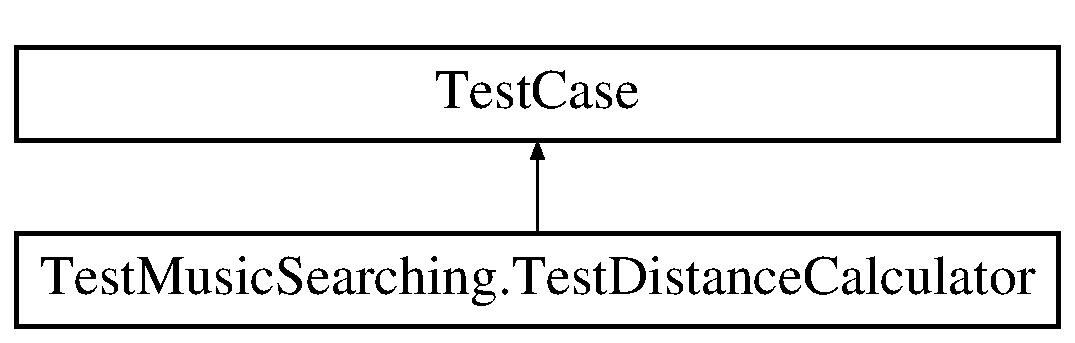
\includegraphics[height=2.000000cm]{class_test_music_searching_1_1_test_distance_calculator}
\end{center}
\end{figure}
\subsection*{Public Member Functions}
\begin{DoxyCompactItemize}
\item 
\mbox{\Hypertarget{class_test_music_searching_1_1_test_distance_calculator_ac37361ea4965452fcffed5ac4e274445}\label{class_test_music_searching_1_1_test_distance_calculator_ac37361ea4965452fcffed5ac4e274445}} 
def {\bfseries test\+\_\+\+Distance} (self)
\end{DoxyCompactItemize}


The documentation for this class was generated from the following file\+:\begin{DoxyCompactItemize}
\item 
Test\+Music\+Searching.\+py\end{DoxyCompactItemize}

\hypertarget{class_test_music_searching_1_1_test_file_operator}{}\section{Test\+Music\+Searching.\+Test\+File\+Operator Class Reference}
\label{class_test_music_searching_1_1_test_file_operator}\index{Test\+Music\+Searching.\+Test\+File\+Operator@{Test\+Music\+Searching.\+Test\+File\+Operator}}
Inheritance diagram for Test\+Music\+Searching.\+Test\+File\+Operator\+:\begin{figure}[H]
\begin{center}
\leavevmode
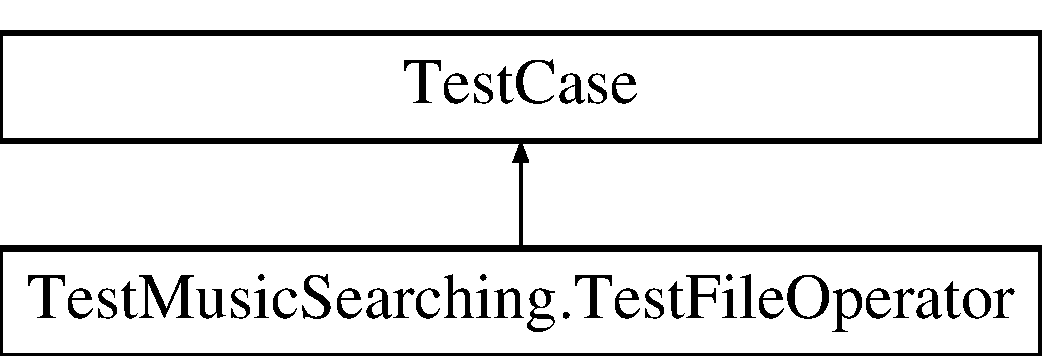
\includegraphics[height=2.000000cm]{class_test_music_searching_1_1_test_file_operator}
\end{center}
\end{figure}
\subsection*{Public Member Functions}
\begin{DoxyCompactItemize}
\item 
\mbox{\Hypertarget{class_test_music_searching_1_1_test_file_operator_a410cfe52ae5d4878490e25e8b715cb46}\label{class_test_music_searching_1_1_test_file_operator_a410cfe52ae5d4878490e25e8b715cb46}} 
def {\bfseries test\+\_\+\+Read\+File} (self)
\item 
\mbox{\Hypertarget{class_test_music_searching_1_1_test_file_operator_abc1e70ea469686a38b1e62de0f431a9e}\label{class_test_music_searching_1_1_test_file_operator_abc1e70ea469686a38b1e62de0f431a9e}} 
def {\bfseries test\+\_\+\+Read\+File\+X\+ML} (self)
\item 
\mbox{\Hypertarget{class_test_music_searching_1_1_test_file_operator_a2d3ed765f4eaf625cdc221d5853bfe09}\label{class_test_music_searching_1_1_test_file_operator_a2d3ed765f4eaf625cdc221d5853bfe09}} 
def {\bfseries test\+\_\+\+Read\+File\+M\+EI} (self)
\item 
\mbox{\Hypertarget{class_test_music_searching_1_1_test_file_operator_a9f620adfa9fe90fbaf37d7d54da9404e}\label{class_test_music_searching_1_1_test_file_operator_a9f620adfa9fe90fbaf37d7d54da9404e}} 
def {\bfseries test\+\_\+\+Save\+Note\+List} (self)
\end{DoxyCompactItemize}


The documentation for this class was generated from the following file\+:\begin{DoxyCompactItemize}
\item 
Test\+Music\+Searching.\+py\end{DoxyCompactItemize}

\hypertarget{class_test_music_searching_1_1_test_seperator}{}\section{Test\+Music\+Searching.\+Test\+Seperator Class Reference}
\label{class_test_music_searching_1_1_test_seperator}\index{Test\+Music\+Searching.\+Test\+Seperator@{Test\+Music\+Searching.\+Test\+Seperator}}
Inheritance diagram for Test\+Music\+Searching.\+Test\+Seperator\+:\begin{figure}[H]
\begin{center}
\leavevmode
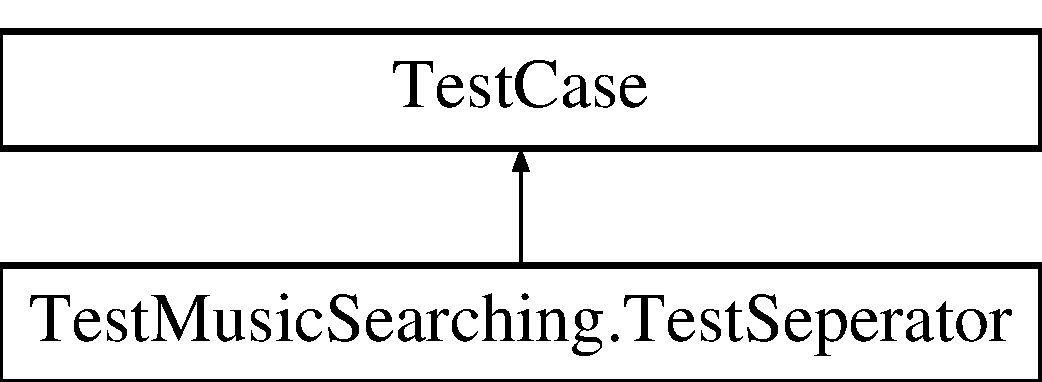
\includegraphics[height=2.000000cm]{class_test_music_searching_1_1_test_seperator}
\end{center}
\end{figure}
\subsection*{Public Member Functions}
\begin{DoxyCompactItemize}
\item 
\mbox{\Hypertarget{class_test_music_searching_1_1_test_seperator_a1ffc8d66e532f85ba827e73603aa40e1}\label{class_test_music_searching_1_1_test_seperator_a1ffc8d66e532f85ba827e73603aa40e1}} 
def {\bfseries test\+\_\+\+Seperate\+By\+Part} (self)
\item 
\mbox{\Hypertarget{class_test_music_searching_1_1_test_seperator_ad0a9181a7b16932ab714ff4d0e212575}\label{class_test_music_searching_1_1_test_seperator_ad0a9181a7b16932ab714ff4d0e212575}} 
def {\bfseries test\+\_\+\+Seperate\+By\+Measure} (self)
\item 
\mbox{\Hypertarget{class_test_music_searching_1_1_test_seperator_a6f24ecd266e3864cb28de530b6a22826}\label{class_test_music_searching_1_1_test_seperator_a6f24ecd266e3864cb28de530b6a22826}} 
def {\bfseries test\+\_\+\+Seperate\+By\+N\+Measure} (self)
\end{DoxyCompactItemize}


The documentation for this class was generated from the following file\+:\begin{DoxyCompactItemize}
\item 
Test\+Music\+Searching.\+py\end{DoxyCompactItemize}

\hypertarget{class_test_music_searching_1_1_test_translator}{}\section{Test\+Music\+Searching.\+Test\+Translator Class Reference}
\label{class_test_music_searching_1_1_test_translator}\index{Test\+Music\+Searching.\+Test\+Translator@{Test\+Music\+Searching.\+Test\+Translator}}
Inheritance diagram for Test\+Music\+Searching.\+Test\+Translator\+:\begin{figure}[H]
\begin{center}
\leavevmode
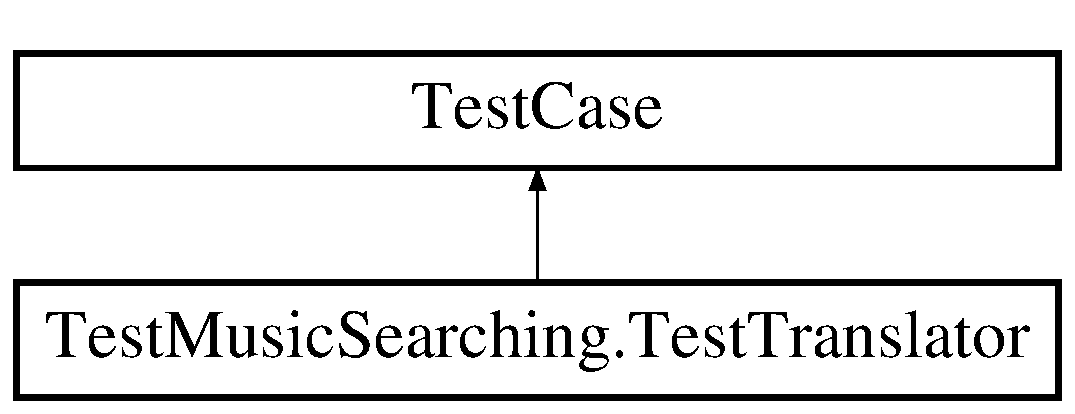
\includegraphics[height=2.000000cm]{class_test_music_searching_1_1_test_translator}
\end{center}
\end{figure}
\subsection*{Public Member Functions}
\begin{DoxyCompactItemize}
\item 
\mbox{\Hypertarget{class_test_music_searching_1_1_test_translator_a9fae337f115752ac5c8ec0f1cd4f931f}\label{class_test_music_searching_1_1_test_translator_a9fae337f115752ac5c8ec0f1cd4f931f}} 
def {\bfseries test\+\_\+\+Translate\+To\+Note} (self)
\item 
\mbox{\Hypertarget{class_test_music_searching_1_1_test_translator_a5ef1be4dfc450fda469027b912bbfa92}\label{class_test_music_searching_1_1_test_translator_a5ef1be4dfc450fda469027b912bbfa92}} 
def {\bfseries test\+\_\+\+Translate\+To\+Note\+List} (self)
\end{DoxyCompactItemize}


The documentation for this class was generated from the following file\+:\begin{DoxyCompactItemize}
\item 
Test\+Music\+Searching.\+py\end{DoxyCompactItemize}

\hypertarget{class_translator_1_1_translator}{}\section{Translator.\+Translator Class Reference}
\label{class_translator_1_1_translator}\index{Translator.\+Translator@{Translator.\+Translator}}
\subsection*{Public Member Functions}
\begin{DoxyCompactItemize}
\item 
def \mbox{\hyperlink{class_translator_1_1_translator_a01afe3034d7b7ce89e397fe024359944}{Translate\+To\+Note}} (self, n, voix)
\item 
def \mbox{\hyperlink{class_translator_1_1_translator_a20b6862fd7e26a69c6eb22fa784b7fe7}{Translate\+To\+Note\+List}} (self, input\+List, voix)
\end{DoxyCompactItemize}


\subsection{Detailed Description}
\begin{DoxyVerb}Operator of the translation of the notes
Translate the note into a list(vector) of number.
Functions:
    TranslateToNote:
    TranslateToNoteList:
\end{DoxyVerb}
 

\subsection{Member Function Documentation}
\mbox{\Hypertarget{class_translator_1_1_translator_a01afe3034d7b7ce89e397fe024359944}\label{class_translator_1_1_translator_a01afe3034d7b7ce89e397fe024359944}} 
\index{Translator\+::\+Translator@{Translator\+::\+Translator}!Translate\+To\+Note@{Translate\+To\+Note}}
\index{Translate\+To\+Note@{Translate\+To\+Note}!Translator\+::\+Translator@{Translator\+::\+Translator}}
\subsubsection{\texorpdfstring{Translate\+To\+Note()}{TranslateToNote()}}
{\footnotesize\ttfamily def Translator.\+Translator.\+Translate\+To\+Note (\begin{DoxyParamCaption}\item[{}]{self,  }\item[{}]{n,  }\item[{}]{voix }\end{DoxyParamCaption})}

\begin{DoxyVerb}Translate a note into a list(vector) of number

This function can Translate a note (format stream.note) into a note (format
Node).

Args:
    n: A node in the musc21.stream
    voix: The part in which exists the note

Returns:
    A note in format Note.
\end{DoxyVerb}
 \mbox{\Hypertarget{class_translator_1_1_translator_a20b6862fd7e26a69c6eb22fa784b7fe7}\label{class_translator_1_1_translator_a20b6862fd7e26a69c6eb22fa784b7fe7}} 
\index{Translator\+::\+Translator@{Translator\+::\+Translator}!Translate\+To\+Note\+List@{Translate\+To\+Note\+List}}
\index{Translate\+To\+Note\+List@{Translate\+To\+Note\+List}!Translator\+::\+Translator@{Translator\+::\+Translator}}
\subsubsection{\texorpdfstring{Translate\+To\+Note\+List()}{TranslateToNoteList()}}
{\footnotesize\ttfamily def Translator.\+Translator.\+Translate\+To\+Note\+List (\begin{DoxyParamCaption}\item[{}]{self,  }\item[{}]{input\+List,  }\item[{}]{voix }\end{DoxyParamCaption})}

\begin{DoxyVerb}Translate a list of notes(in music21.stream) into a list of Notes(format
Note)

This function can Translate a list of notes (format stream.note) into a list
of notes (format Node). It will use the function TranslateToNote to translate
every note in stream and add them into the same list according to the order.

Args:
    inputList: A list of nodes in the musc21.stream
    voix: The part in which exists the notes

Returns:
    A list of notes in format Note.
\end{DoxyVerb}
 

The documentation for this class was generated from the following file\+:\begin{DoxyCompactItemize}
\item 
Translator.\+py\end{DoxyCompactItemize}

%--- End generated contents ---

% Index
\backmatter
\newpage
\phantomsection
\clearemptydoublepage
\addcontentsline{toc}{chapter}{Index}
\printindex

\end{document}
